%%PREAMBLE %%%%%%%%%%%%%%%%%%%%%%%%%%%%
\documentclass[10pt, a4paper]{article}% size of txt = 10pt
\usepackage[top= 2cm,
			bottom = 2cm,
			left = 1.7cm,
			right = 1.7cm,
			footskip = 0.5cm,
			headsep = 0cm,
			headheight = 0cm
					]{geometry}
\usepackage{amsmath} % math packages
\usepackage{amsfonts}% math packages
\usepackage{amssymb} % math packages
\usepackage{graphicx} %package for including graphics
\usepackage{array}
\usepackage[thinlines]{easytable}
\usepackage{float}
\usepackage[section]{placeins}
\usepackage[hidelinks]{hyperref}
\usepackage[shortlabels]{enumitem}
\usepackage{svg}
\usepackage{bigstrut}
\usepackage{wrapfig,lipsum,booktabs}
\usepackage{subcaption}
\usepackage{xfrac}
\usepackage{pdfpages}
\usepackage{listings}
\usepackage{xcolor}

\usepackage{listings}
\usepackage{color} %red, green, blue, yellow, cyan, magenta, black, white
\definecolor{mygreen}{RGB}{28,172,0} % color values Red, Green, Blue
\definecolor{mylilas}{RGB}{170,55,241}

\definecolor{codegreen}{rgb}{0,0.6,0}
\definecolor{codegray}{rgb}{0.5,0.5,0.5}
\definecolor{codepurple}{rgb}{0.58,0,0.82}
\definecolor{backcolour}{rgb}{1,1,1}

\lstdefinestyle{mystyle}{
    backgroundcolor=\color{backcolour},   
    commentstyle=\color{codegreen},
    keywordstyle=\color{magenta},
    numberstyle=\tiny\color{codegray},
    stringstyle=\color{codepurple},
    basicstyle=\ttfamily\footnotesize,
    breakatwhitespace=false,         
    breaklines=true,                 
    captionpos=b,                    
    keepspaces=true,                 
    numbers=left,                    
    numbersep=5pt,                  
    showspaces=false,                
    showstringspaces=false,
    showtabs=false,                  
    tabsize=2
}
\lstset{style=mystyle}


%date format
\def\mydate{\leavevmode\hbox{\twodigits\day.\twodigits\month.\the\year}}
\def\twodigits#1{\ifnum#1<10 0\fi\the#1}


\usepackage[T1]{fontenc} 
\usepackage{lmodern}
\usepackage{indentfirst}
\setlength{\parindent}{1cm}

\makeatletter
\newcommand{\thickhline}{%
    \noalign {\ifnum 0=`}\fi \hrule height 2pt
    \futurelet \reserved@a \@xhline
}
\newcolumntype{"}{@{\hskip\tabcolsep\vrule width 2pt\hskip\tabcolsep}}
\makeatother
\newcolumntype{?}{!{\vrule width 2pt}}
%%DOC ENVIROMENT%%%%%%%%%%%%%%%%%%%%%%%
\begin{document}
%Title 
\begin{flushleft}%% left justification
	\textbf{\Large{MKC-KVE: Laboratorní úloha č. 4}}\hfill Filip Paul\\
	\large{Měření světelné charakteristiky laserové diody a LED \hfill 14.10.2022}
\end{flushleft}
	\section{\Large Naměřená W/A a V/A charakteristika pro laserovou diodu:}
	\begin{figure}[ht!]
		\centering
		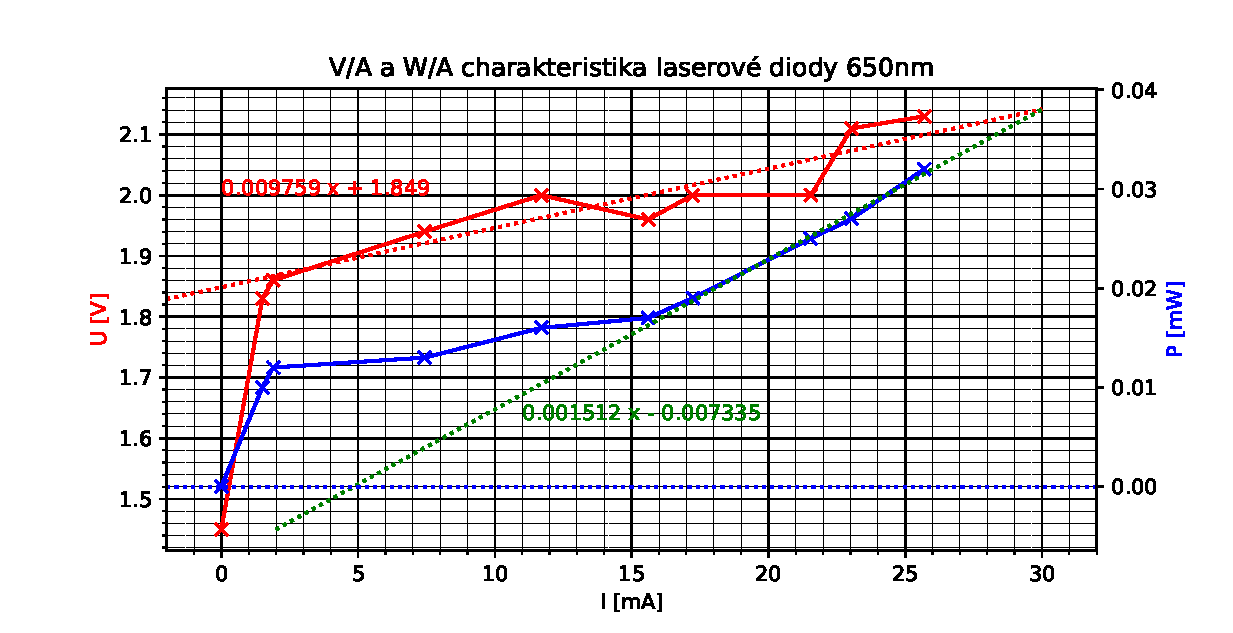
\includegraphics[width = 1\textwidth]{Laser_650nm.eps}
	\end{figure}

	Z naměřených výsledků W/A charakteristiky laserové diody bohužel nelze spolehlivě určit prahovou hodnotu budícího proudu
	$I_{b}$, pravděpodobně z důvodu, že laserová dioda už na konci životního cyklu.
	Dále naměřený optický výkon laserové diody byl velmi nízký (řádově desítky $\mu$W).
	Nejsem si úplně jistý, zda měřič optického výkonu byl správně nastaven, protože
	oproti měření LED měla laserová dioda mnohem nižší hodnoty vyzařovaného optického výkonu
	a to i přestože byl paprsek laserové diody jasně viditelný.\\

	Při měření laserové diody byl paprsek již okem viditelný okolo budícího proudu 1.5\,mA.
	Pro určení $I_{b}$ z měřených dat byly výsledné data proloženy lineární křivkou (zeleně), přičemž bylo
	pro aproximaci zvoleno posledních 5 naměřených dat, z důvodu že tato část vypadá nejlineárněji.
	$I_{b}$ lze přibližně určit jako 5\,mA. Pokud bychom vyšli ze stejné úvahy, že pro posledních 5
	naměřených hodnot je charakteristika nejlineárnější, $I_{bmin}$ by se pak rovnal 15\,mA.
	Přičemž tomuto proudu odpovídá vyzařovaný optický výkon 17\,$\mu W$.
	Koeficient konverze $k_I$ je patrný z funkčního předpisu zelené křivky a je roven 0.001512.\\
	
	Obdobně lze určit i dynamický odpor laserové diody nyní však s předpisu funkce pro červenou křivku,
	která vznikla proložením "lineární"\ části V/A charakteristiky. Dynamický odpor je pak roven
	9.750$\Omega$. Obdobným způsobem byly zjištěny dynamické odporu u měřených LED diod. Postup určení
	parametrů diod se pak pouze liší ve výběru naměřených dat, z kterých jsou vytvořeny lineární aproximace.
	Na konci dokumentu je souhrn výsledků.

	\begin{figure}[ht!]
		\centering
		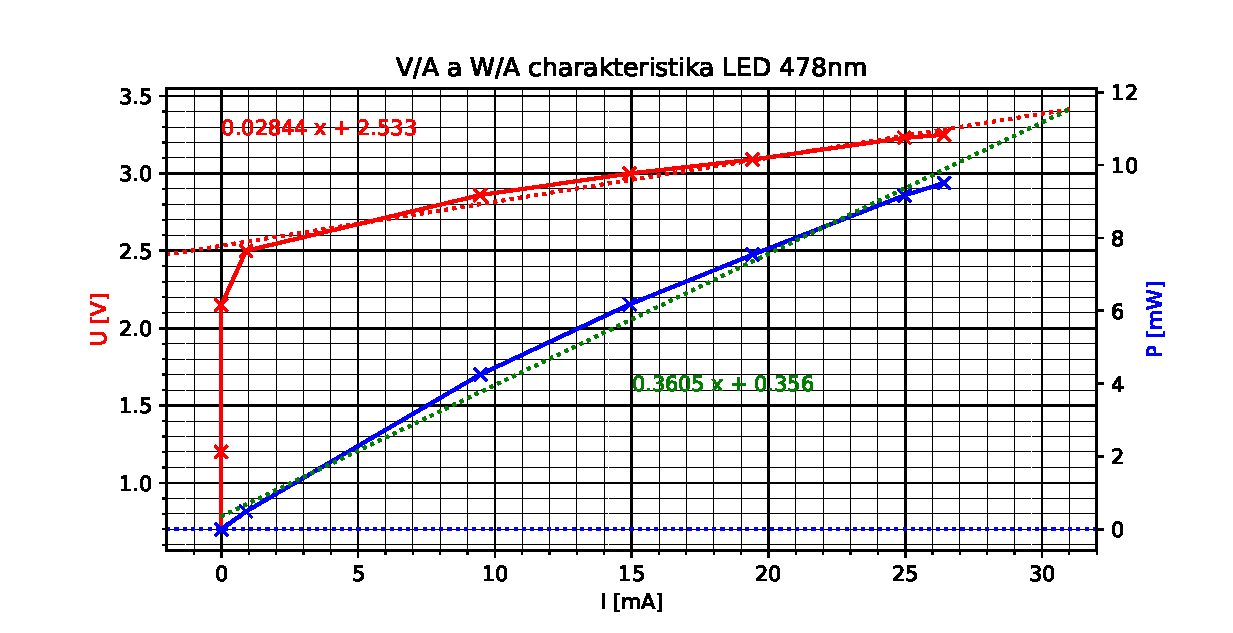
\includegraphics[width = 0.95\textwidth]{LED_478nm.eps}
		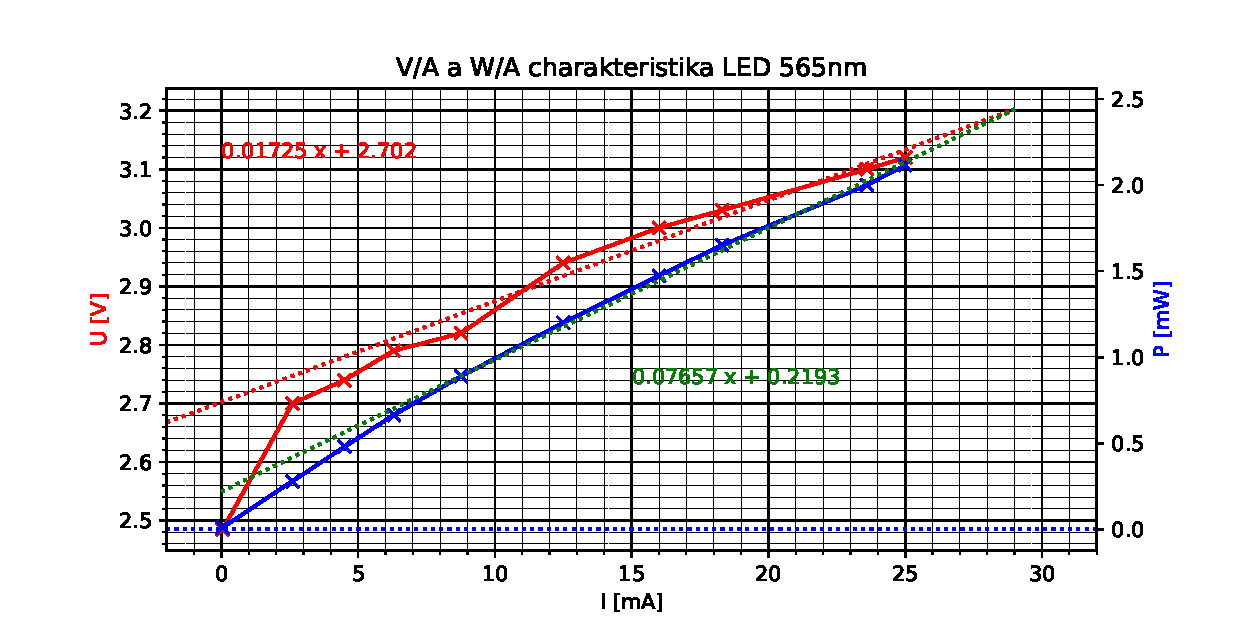
\includegraphics[width = 0.95\textwidth]{LED_565nm.eps}
		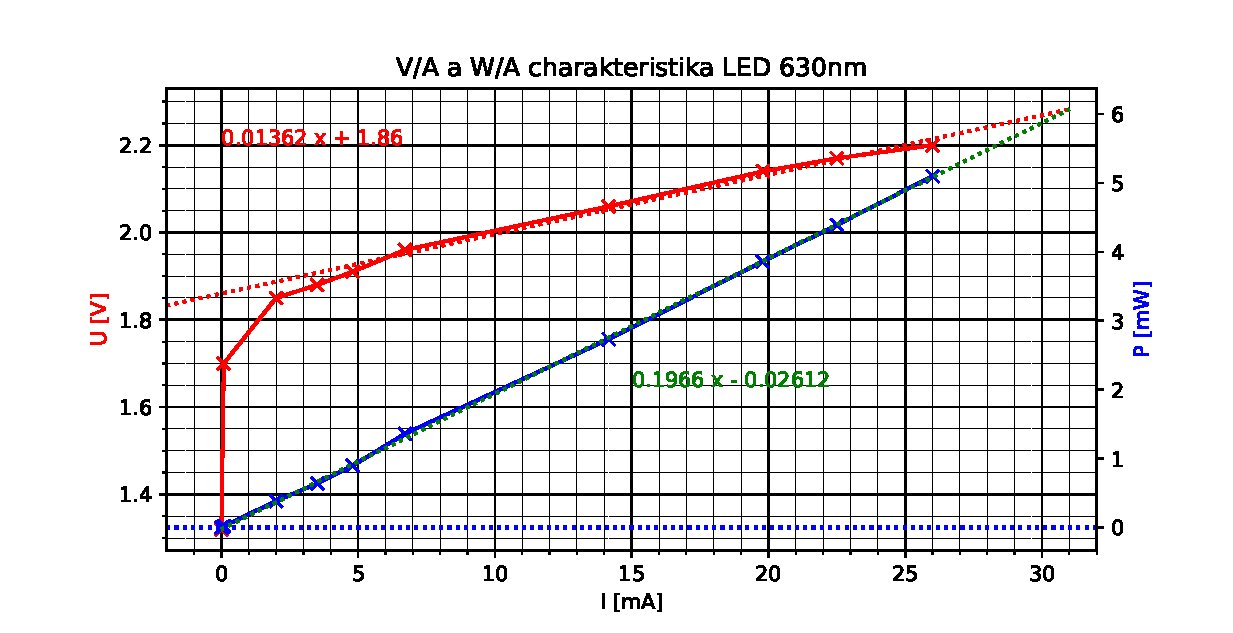
\includegraphics[width = 0.95\textwidth]{LED_630nm.eps}
	\end{figure}


	\clearpage
	\section{\Large Souhrn výsledků:}
	\begin{table}[ht!]
		\resizebox{0.3\columnwidth}{!}{%
		\begin{tabular}{|l|l|l|}
		\hline
		\textbf{$\lambda$ {[}nm{]}} & \textbf{kI{[}W/A{]}} & \textbf{rd {[}$\Omega${]}} \\ \hline
		650 (laser)              & 0.001512             & 9.759                      \\ \hline
		478                      & 0.3605               & 28.4                       \\ \hline
		565                      & 0.07657              & 17.25                      \\ \hline
		630                      & 0.1966               & 13.62                      \\ \hline
		\end{tabular}%
		}
	\end{table}

	$I_{b}$ pro laserovou diodou: 5\,mA.



		
	%\end{figure}
%
	%\begin{figure}[ht!]
	%		\centering
	%	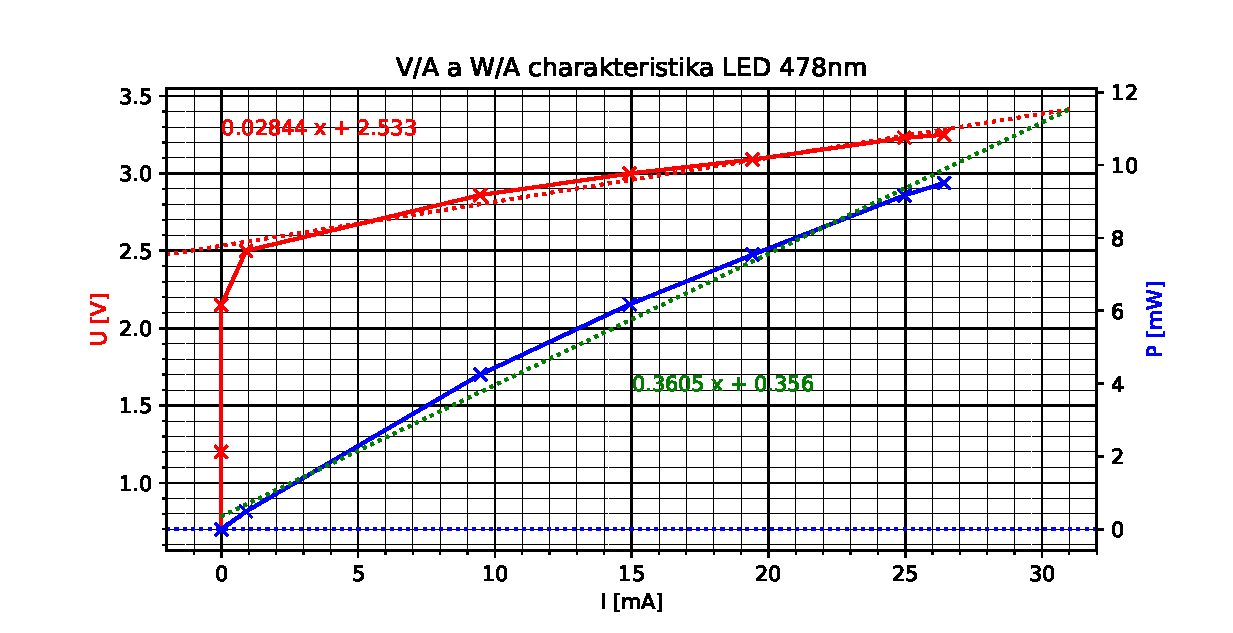
\includegraphics[width = 1\textwidth]{LED_478nm.eps}
	%	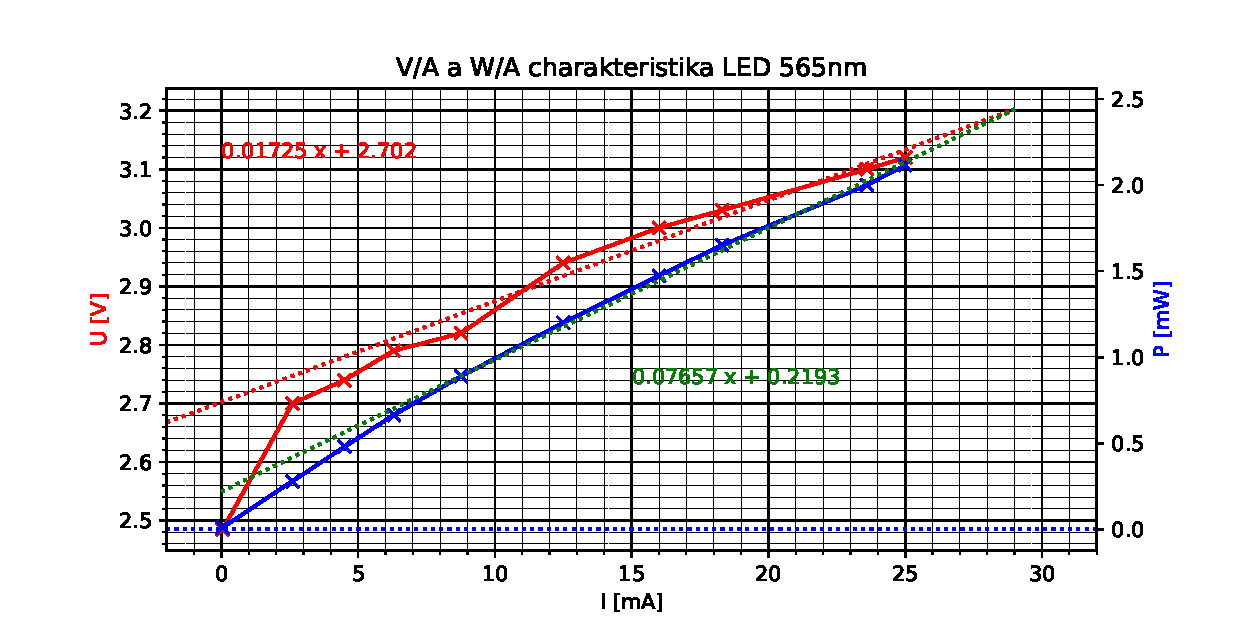
\includegraphics[width = 1\textwidth]{LED_565nm.eps}
	%	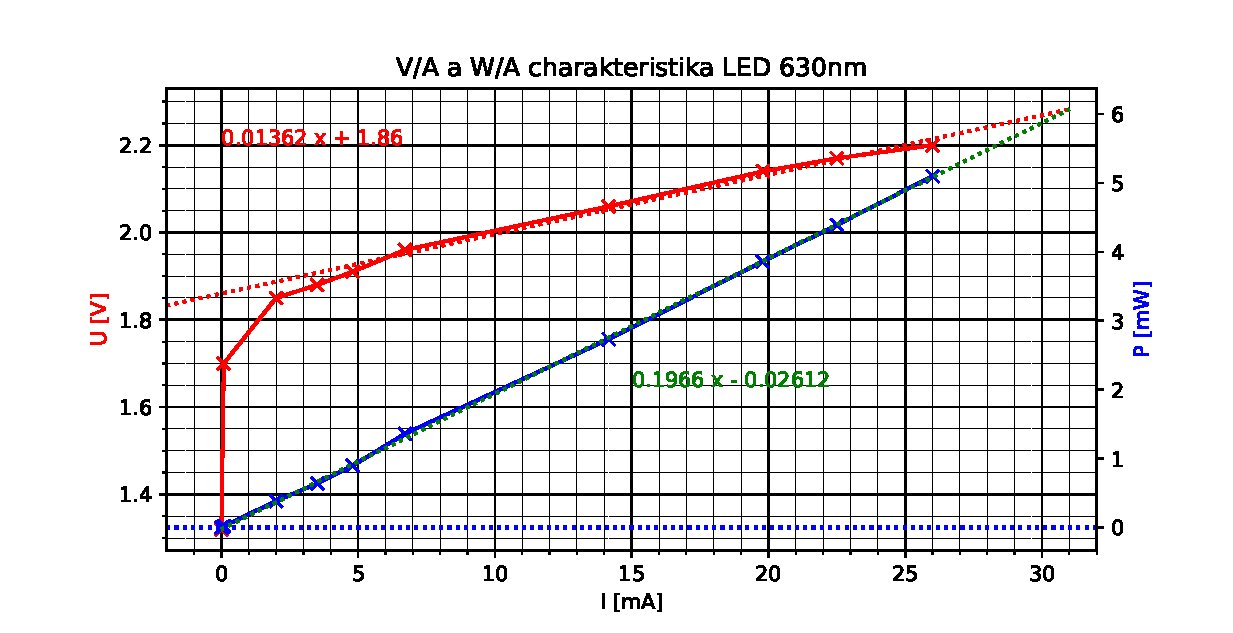
\includegraphics[width = 1\textwidth]{LED_630nm.eps}
	%	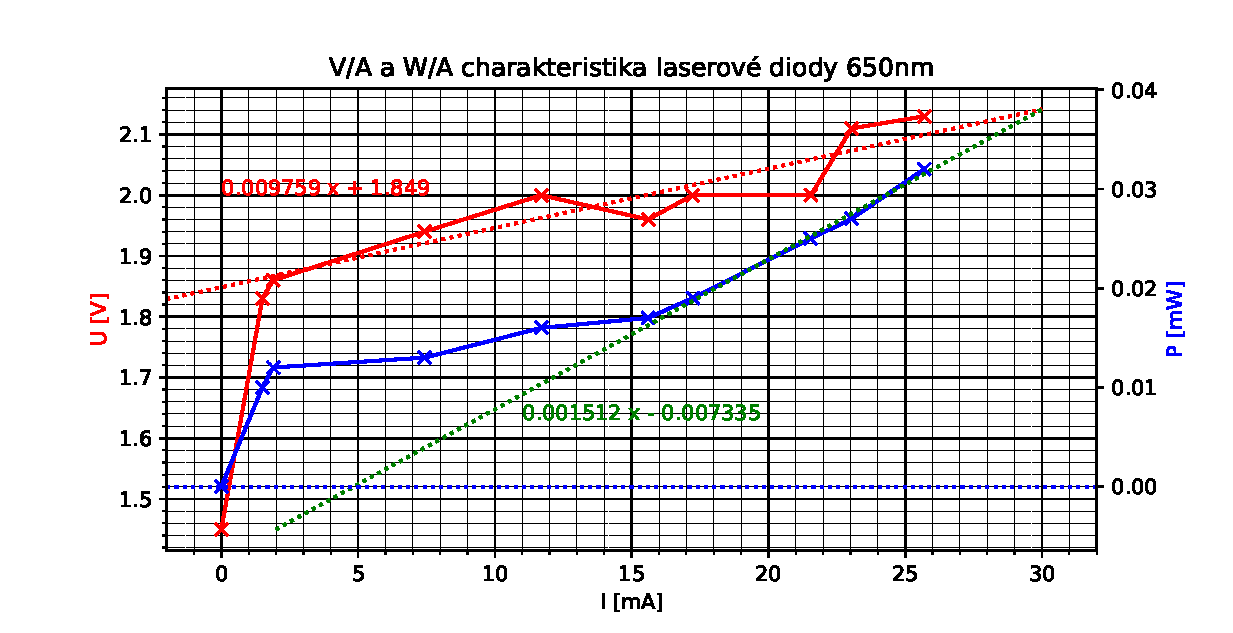
\includegraphics[width = 1\textwidth]{Laser_650nm.eps}
	%\end{figure}



\end{document}


%\[f(x)= (x+2)^2 - \frac{9\cdot 2\pi}{26}\] %%mathematic equatation in display style mode
%%optional:
%	\begin{align} %%this alignes all charakters after & if *is removed equations will be numbered
%	\hspace{5cm}  
%		 x &= a_2 x^2 +_1 x + a_0 \\
% 		x &=x^2 \nonumber		%no number will not add number to eq
%	\end{align}
